\documentclass[aspectratio=169,11pt]{beamer}
\usetheme{default}
\usefonttheme{professionalfonts}
\setbeamertemplate{navigation symbols}{}
\setbeamertemplate{footline}[frame number]
\setbeamercolor{normal text}{fg=black,bg=white}
\setbeamercolor{structure}{fg=black}
\setbeamercolor{frametitle}{fg=black,bg=white}
\setbeamertemplate{itemize item}{\textbullet}
\usepackage{fontspec}
\IfFontExistsTF{Arial}{\setsansfont{Arial}}{\setsansfont{Arimo}}
\usepackage{graphicx}
\graphicspath{{../diagrams/}}
\title{CS341 Software Engineering: Task Tracker}
\subtitle{Project 1 --- Plain English Project Presentation}
\date{1 November 2026}
\begin{document}
\begin{frame}\titlepage\end{frame}
\begin{frame}{Problem and Scope}\begin{itemize}\item Small teams need to assign and track tasks.\item Single-machine Java desktop application.\item Multiple accounts use one local SQLite file.\item No real-time online synchronization.\end{itemize}\end{frame}
\begin{frame}{Assignment Requirements}\begin{itemize}\item Register, log in and log out.\item Create, assign, edit, delete and complete tasks.\item View created or assigned tasks.\item Persist data with SQLite through JDBC.\item Use Git, JUnit 5 and documented system design.\end{itemize}\end{frame}
\begin{frame}{Additional Features}\begin{itemize}\item Three priority levels: LOW, MEDIUM, HIGH.\item Optional due dates in YYYY-MM-DD format.\item Open / completed / high-priority filters.\item Sorting by task table columns.\end{itemize}\end{frame}
\begin{frame}{Use Cases}\centering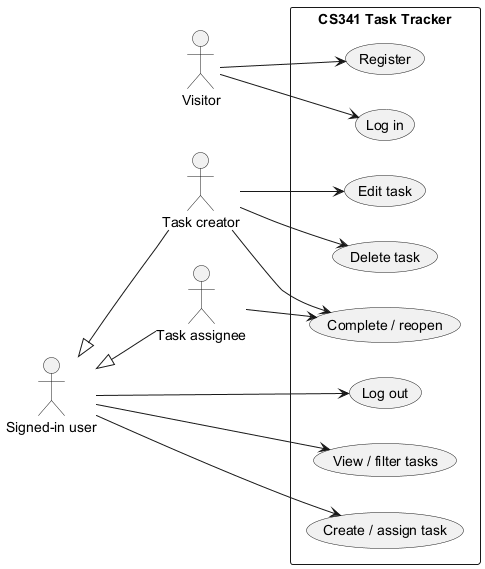
\includegraphics[width=.92\linewidth,height=.75\textheight,keepaspectratio]{use_case.png}\end{frame}
\begin{frame}{Architecture}\begin{itemize}\item Swing View: MainFrame.\item Controller: TaskTrackerController.\item Business rules: AuthService and TaskService.\item Storage access: repositories and Database.\end{itemize}\end{frame}
\begin{frame}{Class Diagram}\centering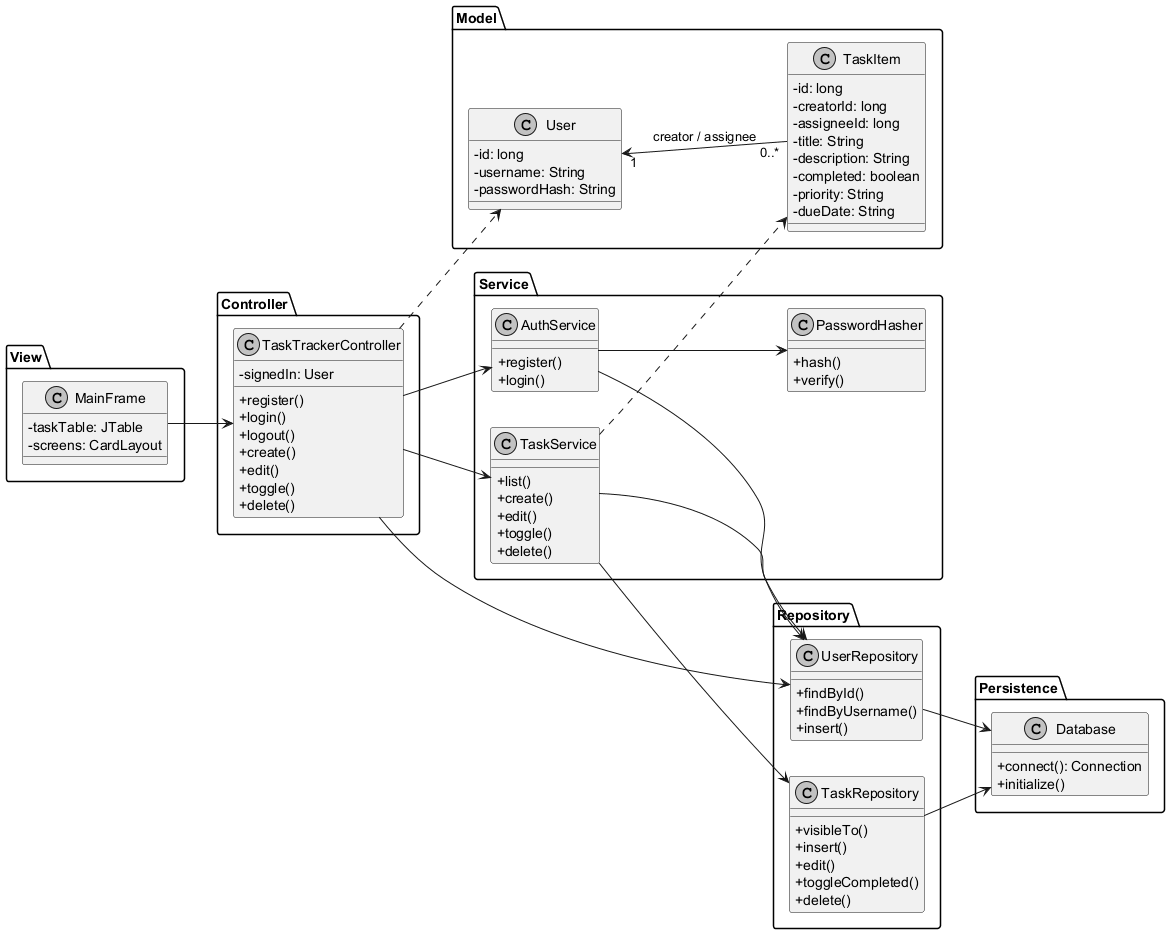
\includegraphics[width=.97\linewidth,height=.76\textheight,keepaspectratio]{class.png}\end{frame}
\begin{frame}{SQLite Data Model}\centering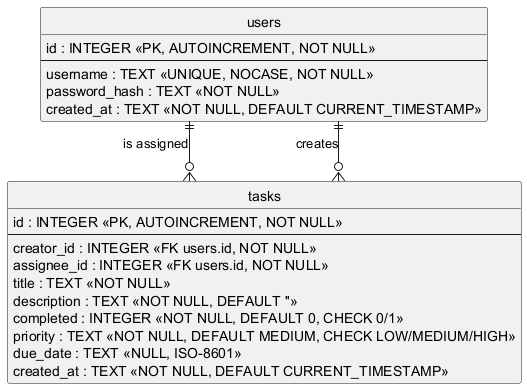
\includegraphics[width=.9\linewidth,height=.74\textheight,keepaspectratio]{er.png}\end{frame}
\begin{frame}{Authorization}\begin{itemize}\item Creator: view, edit, delete and toggle completion.\item Assignee: view and toggle completion.\item Unrelated user: no access.\item SQL writes have user-ID conditions as a second guard.\end{itemize}\end{frame}
\begin{frame}{Task Completion Sequence}\centering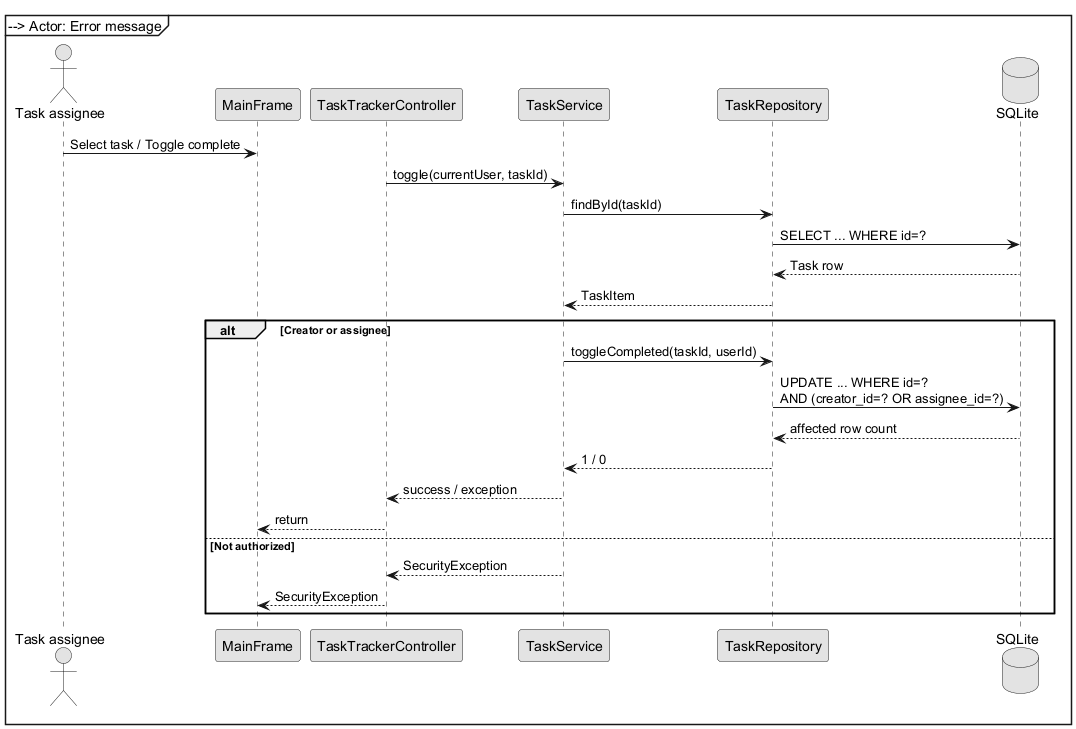
\includegraphics[width=.88\linewidth,height=.73\textheight,keepaspectratio]{sequence.png}\end{frame}
\begin{frame}{Implementation Details}\begin{itemize}\item Java 11+, Swing, JDBC and SQLite.\item Parameterized SQL and database foreign keys.\item Salted PBKDF2 password hashes.\item Automatic creation of users and tasks tables.\end{itemize}\end{frame}
\begin{frame}{Automated Tests}\begin{itemize}\item Maven/Surefire: 17 JUnit 5 tests passed; 0 failures, errors or skips.\item Packaged JAR SQLite JDBC create/insert/read smoke test passed.\item Independent Python SQLite checks: 10/10 passed.\item Final ZIP extracted and passed a clean Maven build.\end{itemize}\end{frame}
\begin{frame}{Manual Demo Script}\begin{enumerate}\item Register Alice and Bob.\item Alice assigns a task to Bob.\item Bob completes the task but cannot edit/delete.\item Alice changes priority, reassigns or deletes the task.\item Restart: verify persistence and task filters.\end{enumerate}\end{frame}
\begin{frame}{Design Trade-offs}\begin{itemize}\item Local database: low setup cost, offline use.\item No multi-device collaboration or backup automation.\item Permission policy is a stated design choice.\item Lean MVC-oriented packages for small-coursework scope.\end{itemize}\end{frame}
\begin{frame}{Open Verification Gates}\begin{itemize}\item Run AT-01--AT-08 on a real desktop and capture genuine GUI evidence.\item Provide authentic 3--4 member contributions and Git history.\item Publish only with team approval and record the real remote CI result.\item Deliver the live demo with all actual team members.\end{itemize}\end{frame}
\begin{frame}{Conclusion}\begin{itemize}\item Local Maven/JUnit/JDBC, packaged-JAR SQLite and extracted ZIP builds passed.\item Seven PlantUML sources were rendered; six English PDFs were rebuilt.\item GUI acceptance and real team/GitHub submission remain open.\end{itemize}\vspace{1em}\centering\large Questions?\end{frame}
\end{document}
